\documentclass[12pt,twoside]{article}
\usepackage{minted}
\usepackage[dvipsnames]{xcolor}
\usepackage{tikz,graphicx,amsmath,amsfonts,amscd,amssymb,bm,cite,epsfig,epsf,url}
\usepackage[hang,flushmargin]{footmisc}
\usepackage[colorlinks=true,urlcolor=blue,citecolor=blue]{hyperref}
\usepackage{amsthm,multirow,wasysym,appendix}
\usepackage{array,subcaption} 
% \usepackage[small,bf]{caption}
\usepackage{bbm}
\usepackage{pgfplots}
\usetikzlibrary{spy}
\usepgfplotslibrary{external}
\usepgfplotslibrary{fillbetween}
\usetikzlibrary{arrows,automata}
\usepackage{thmtools}
\usepackage{blkarray} 
\usepackage{textcomp}
\usepackage[left=0.8in,right=1.0in,top=1.0in,bottom=1.0in]{geometry}
\usepackage{pifont}
\usepackage{tikz-qtree}

%% Probability operators and functions
%
% \def \P{\mathrm{P}}
\def \P{\mathrm{P}}
\def \E{\mathrm{E}}
\def \Var{\mathrm{Var}}
\let\var\Var
\def \Cov {\mathrm{Cov}} \let\cov\Cov
\def \MSE {\mathrm{MSE}} \let\mse\MSE
\def \sgn {\mathrm{sgn}}
\def \R {\mathbb{R}}
\def \C {\mathbb{C}}
\def \N {\mathbb{N}}
\def \Z {\mathbb{Z}}
\def \cV {\mathcal{V}}
\def \cS {\mathcal{S}}

\newcommand{\RR}{\ensuremath{\mathbb{R}}}

\DeclareMathOperator*{\argmin}{arg\,min}
\DeclareMathOperator*{\argmax}{arg\,max}
\newcommand{\red}[1]{\textcolor{red}{#1}}
\newcommand{\blue}[1]{\textcolor{blue}{#1}}
\newcommand{\green}[1]{\textcolor{ForestGreen}{ #1}}
\newcommand{\fuchsia}[1]{\textcolor{RoyalPurple}{ #1}}



%
%% Probability distributions
%
%\def \Bern    {\mathrm{Bern}}
%\def \Binom   {\mathrm{Binom}}
%\def \Exp     {\mathrm{Exp}}
%\def \Geom    {\mathrm{Geom}}
% \def \Norm    {\mathcal{N}}
%\def \Poisson {\mathrm{Poisson}}
%\def \Unif    {\mathrm {U}}
%
\DeclareMathOperator{\Norm}{\mathcal{N}}

\newcommand{\bdb}[1]{\textcolor{red}{#1}}

\newcommand{\ml}[1]{\mathcal{ #1 } }
\newcommand{\wh}[1]{\widehat{ #1 } }
\newcommand{\wt}[1]{\widetilde{ #1 } }
\newcommand{\conj}[1]{\overline{ #1 } }
\newcommand{\rnd}[1]{\tilde{ #1 } }
\newcommand{\rv}[1]{ \rnd{ #1}  }
\newcommand{\rM}{\rnd{ m}  }
\newcommand{\rx}{\rnd{ x}  }
\newcommand{\ry}{\rnd{ y}  }
\newcommand{\rz}{\rnd{ z}  }
\newcommand{\ra}{\rnd{ a}  }
\newcommand{\rb}{\rnd{ b}  }
\newcommand{\rt}{\rnd{ t}  }
\newcommand{\rs}{\rnd{ s}  }


\newcommand{\rpc}{\widetilde{ pc}  }
\newcommand{\rndvec}[1]{\vec{\rnd{#1}}}

\def \cnd {\, | \,}
\def \Id { I }
\def \J {\mathbf{1}\mathbf{1}^T}

\newcommand{\op}[1]{\operatorname{#1}}
\newcommand{\setdef}[2]{ := \keys{ #1 \; | \; #2 } }
\newcommand{\set}[2]{ \keys{ #1 \; | \; #2 } }
\newcommand{\sign}[1]{\op{sign}\left( #1 \right) }
\newcommand{\trace}[1]{\op{tr}\left( #1 \right) }
\newcommand{\tr}[1]{\op{tr}\left( #1 \right) }
\newcommand{\inv}[1]{\left( #1 \right)^{-1} }
\newcommand{\abs}[1]{\left| #1 \right|}
\newcommand{\sabs}[1]{| #1 |}
\newcommand{\keys}[1]{\left\{ #1 \right\}}
\newcommand{\sqbr}[1]{\left[ #1 \right]}
\newcommand{\sbrac}[1]{ ( #1 ) }
\newcommand{\brac}[1]{\left( #1 \right) }
\newcommand{\bbrac}[1]{\big( #1 \big) }
\newcommand{\Bbrac}[1]{\Big( #1 \Big)}
\newcommand{\BBbrac}[1]{\BIG( #1 \Big)}
\newcommand{\MAT}[1]{\begin{bmatrix} #1 \end{bmatrix}}
\newcommand{\sMAT}[1]{\left(\begin{smallmatrix} #1 \end{smallmatrix}\right)}
\newcommand{\sMATn}[1]{\begin{smallmatrix} #1 \end{smallmatrix}}
\newcommand{\PROD}[2]{\left \langle #1, #2\right \rangle}
\newcommand{\PRODs}[2]{\langle #1, #2 \rangle}
\newcommand{\der}[2]{\frac{\text{d}#2}{\text{d}#1}}
\newcommand{\pder}[2]{\frac{\partial#2}{\partial#1}}
\newcommand{\derTwo}[2]{\frac{\text{d}^2#2}{\text{d}#1^2}}
\newcommand{\ceil}[1]{\lceil #1 \rceil}
\newcommand{\Imag}[1]{\op{Im}\brac{ #1 }}
\newcommand{\Real}[1]{\op{Re}\brac{ #1 }}
\newcommand{\norm}[1]{\left|\left| #1 \right|\right| }
\newcommand{\norms}[1]{ \| #1 \|  }
\newcommand{\normProd}[1]{\left|\left| #1 \right|\right| _{\PROD{\cdot}{\cdot}} }
\newcommand{\normTwo}[1]{\left|\left| #1 \right|\right| _{2} }
\newcommand{\normTwos}[1]{ \| #1  \| _{2} }
\newcommand{\normZero}[1]{\left|\left| #1 \right|\right| _{0} }
\newcommand{\normTV}[1]{\left|\left| #1 \right|\right|  _{ \op{TV}  } }% _{\op{c} \ell_1} }
\newcommand{\normOne}[1]{\left|\left| #1 \right|\right| _{1} }
\newcommand{\normOnes}[1]{\| #1 \| _{1} }
\newcommand{\normOneTwo}[1]{\left|\left| #1 \right|\right| _{1,2} }
\newcommand{\normF}[1]{\left|\left| #1 \right|\right| _{\op{F}} }
\newcommand{\normLTwo}[1]{\left|\left| #1 \right|\right| _{\ml{L}_2} }
\newcommand{\normNuc}[1]{\left|\left| #1 \right|\right| _{\ast} }
\newcommand{\normOp}[1]{\left|\left| #1 \right|\right|  }
\newcommand{\normInf}[1]{\left|\left| #1 \right|\right| _{\infty}  }
\newcommand{\proj}[1]{\mathcal{P}_{#1} \, }
\newcommand{\diff}[1]{ \, \text{d}#1 }
\newcommand{\vc}[1]{\boldsymbol{\vec{#1}}}
\newcommand{\rc}[1]{\boldsymbol{#1}}
\newcommand{\vx}{\vec{x}}
\newcommand{\vy}{\vec{y}}
\newcommand{\vz}{\vec{z}}
\newcommand{\vu}{\vec{u}}
\newcommand{\vv}{\vec{v}}
\newcommand{\vb}{\vec{\beta}}
\newcommand{\va}{\vec{\alpha}}
\newcommand{\vaa}{\vec{a}}
\newcommand{\vbb}{\vec{b}}
\newcommand{\vg}{\vec{g}}
\newcommand{\vw}{\vec{w}}
\newcommand{\vh}{\vec{h}}
\newcommand{\vbeta}{\vec{\beta}}
\newcommand{\valpha}{\vec{\alpha}}
\newcommand{\vgamma}{\vec{\gamma}}
\newcommand{\veta}{\vec{\eta}}
\newcommand{\vnu}{\vec{\nu}}
\newcommand{\rw}{\rnd{w}}
\newcommand{\rvnu}{\vc{\nu}}
\newcommand{\rvv}{\rndvec{v}}
\newcommand{\rvw}{\rndvec{w}}
\newcommand{\rvx}{\rndvec{x}}
\newcommand{\rvy}{\rndvec{y}}
\newcommand{\rvz}{\rndvec{z}}
\newcommand{\rvX}{\rndvec{X}}


\newtheorem{theorem}{Theorem}[section]
% \declaretheorem[style=plain,qed=$\square$]{theorem}
\newtheorem{corollary}[theorem]{Corollary}
\newtheorem{definition}[theorem]{Definition}
\newtheorem{lemma}[theorem]{Lemma}
\newtheorem{remark}[theorem]{Remark}
\newtheorem{algorithm}[theorem]{Algorithm}

% \theoremstyle{definition}
%\newtheorem{example}[proof]{Example}
\declaretheorem[style=definition,qed=$\triangle$,sibling=definition]{example}
\declaretheorem[style=definition,qed=$\bigcirc$,sibling=definition]{application}

%
%% Typographic tweaks and miscellaneous
%\newcommand{\sfrac}[2]{\mbox{\small$\displaystyle\frac{#1}{#2}$}}
%\newcommand{\suchthat}{\kern0.1em{:}\kern0.3em}
%\newcommand{\qqquad}{\kern3em}
%\newcommand{\cond}{\,|\,}
%\def\Matlab{\textsc{Matlab}}
%\newcommand{\displayskip}[1]{\abovedisplayskip #1\belowdisplayskip #1}
%\newcommand{\term}[1]{\emph{#1}}
%\renewcommand{\implies}{\;\Rightarrow\;}



\begin{document}

\begin{center}
{\large{\textbf{Homework 8}} } \vspace{0.2cm}\\
Due Apr 2 at 11 pm
\\
\end{center}
Unless stated otherwise, justify any answers you give.
You can work in groups, but each
student must write their own solution based on their own
understanding of the problem.

When uploading your homework to Gradescope you will have to
select the relevant pages for each question.  Please submit each
problem on a separate page (i.e., 1a and~1b can be on the same page but 1
and 2 must be on different pages).  We understand that this may be
cumbersome but this is the best way for the grading team to grade your
homework assignments and provide feedback in a timely manner.  Failure
to adhere to these guidelines may result in a loss of points.
Note that it may take some time to
select the pages for your submission.  Please plan accordingly.  We
suggest uploading your assignment at least 30 minutes before the deadline
so you will have ample time to select the correct pages for your
submission.  If you are using \LaTeX, consider using the minted or
listings packages for typesetting code.  
\\

\begin{enumerate}

\item (Random vector) 
A random vector $\rx$ with zero mean has a covariance matrix $\Sigma_{\rx}$ with the following eigendecomposition
\begin{align}
\Sigma_{\rx} = \MAT{1 & 0 & 0 \\ 0 & \frac{1}{\sqrt{2}} & \frac{1}{\sqrt{2}} \\ 0 & \frac{1}{\sqrt{2}} & -\frac{1}{\sqrt{2}}} \MAT{1 & 0 & 0 \\ 0 & 0.5 & 0 \\ 0 & 0 & 0} \MAT{1 & 0 & 0 \\ 0 & \frac{1}{\sqrt{2}} & \frac{1}{\sqrt{2}} \\ 0 & \frac{1}{\sqrt{2}} & -\frac{1}{\sqrt{2}}}.
\end{align}
\begin{enumerate}
\item What is the variance of each of the entries of the random vector $\rx[1]$, $\rx[2]$ and $\rx[3]$?
\begin{itemize}
  \color{blue}
  \item we know that the variance of the enteries of a random vector x are the diagnoal enteries of it's covariance matrix 
  \item so in this case as we are given an eigendecomposition of the form $Q\lambda Q^{-1}=\Sigma_{\Tilde{x}}$
  \item we can compute $\Sigma_{\Tilde{x}}=\begin{pmatrix}
    1 & 0 &0\\
    0 & \frac{1}{4} & \frac{1}{4}\\
    0 & \frac{1}{4} & \frac{1}{4}\\
  \end{pmatrix}$
  \item so thus we can see $var(\Tilde{x}[1])=1$ and $var(\Tilde{x}[2])=var(\Tilde{x}[3])=\frac{1}{4}$
\end{itemize}

\item Is it possible to find a unit-norm vector $u$ such that the inner product between $\rx$ and $u$ (i.e. the amplitude of the projection of $\rx$ onto that direction) has variance greater than 1?
\begin{itemize}
  \color{blue}
  \item we can write the variance of any linear combination of $\Tilde{x}$ and a vector $a\in \mathbb{R}^{d}$ as $var(a^t\Tilde{x})=a^t\Sigma_{\Tilde{x}}a$
  \item doing this out for an arbitrary vector $a=\begin{pmatrix}
    a_1\\1_2\\1_3
  \end{pmatrix}$ we can see that $j(a)=a^t\Sigma_{\Tilde{x}}a$
  \item we know we are looking for the max such that a has unit norm so we can write this as a lagrangian 
  \item $max_{a\in \mathbb{R}^{3}}j(a) \text{ such that} ||a||=1\iff max(\mathcal{L}(a,\lambda ))=max_{a,\lambda}j(a)-\lambda(||a||-1)$
  \item so now to maximize we can find $\frac{\partial \mathcal{L}}{\partial a}=2a^t\Sigma_{\Tilde{x}}-2\lambda a\Rightarrow a^t\Sigma_{\Tilde{x}}=\lambda a$ so in other words our function max must be achieved when $a$ is an eigen vector of $\Sigma_{\Tilde{x}}$  
  \item then we can find  $\frac{\partial \mathcal{L}}{\partial \lambda}=||a||-1=0\rightarrow ||a||=1$ie at the max a must have unit norm
  \item this gives us three canaanite points (the three eigenvectors ie columns of $Q$)
  \item  doing this out we can see $j(\begin{pmatrix}
    1\\0\\0
  \end{pmatrix})=1,j(\begin{pmatrix}
    0\\\frac{1}{\sqrt{2}}\\\frac{1}{\sqrt{2}}
  \end{pmatrix})=.5,j(\begin{pmatrix}
    0\\\frac{1}{\sqrt{2}}\\-\frac{1}{\sqrt{2}}
  \end{pmatrix})=0$
  \item thus no we can never have a linear combination $\Tilde{x}$ and some vector a with variance greater than 1. 


\end{itemize}
\item Find three constants $a_1$, $a_2$ and $a_3$, such that at least one of them is nonzero and $\P(a_1 \rx[1]+ a_2 \rx[2] + a_3 \rx[3] = 0) = 1$. Justify your answer mathematically, and interpret it geometrically.  
\begin{itemize}
  \color{blue}
  \item we know a random variable with 0 variance will always equal it's mean 
  \item we know that for any vector $a\in \mathbb{R}^{3}$ by the properties of gaussian random vectors $E[a^t\Tilde{x}]=a^tE[\tilde{x}]=0$
  \item so in other words for our linear combination $a^t\Tilde{x}$ to always equal zero we just need to find any vector a such that $var(a^t\Tilde{x})=0$
  \item we know that $var(a^{t}\Tilde{x})=a^{t}\Sigma_{\Tilde{x}}a$ we showed in the last problem that 
  \item $a^{t}\Sigma_{\Tilde{x}}a=0$ when $a=\begin{pmatrix}
    0\\\frac{1}{\sqrt{2}}\\-\frac{1}{\sqrt{2}}
  \end{pmatrix}$ 
  \item geometrically this makes sense as  $a=\begin{pmatrix}
    0\\\frac{1}{\sqrt{2}}\\-\frac{1}{\sqrt{2}}
  \end{pmatrix}$  is an eigenvecotr of $\Sigma_{\Tilde{x}}$ associated to eigen value 0 so in other words, it is an eigenvalue in the null space of our covariance matrix 
\end{itemize}

\end{enumerate}
\newpage
\item (Basketball team) The coach of a basketball needs to choose two out of three players to play as guards during the last quarter of a game. The covariance matrix of the points scored by the players in a quarter is the following
 \begin{center}
\begin{tabular}{ | c | c | c | c |  } % c | c | c l c | c | c | c | c | c | }
  \hline			
&  Player A & Player B & Player C \\
  \hline			
Player A & 100 & -80 & 10   \\
  \hline  
Player B  & -80  & 81 & 50 \\ 
  \hline  
Player C &  10 & 50 & 100\\
 \hline  
 \end{tabular} .
\end{center}
Compute the variance of the total number of points if the coach plays the three possible combinations of two players. Assuming all three players score the same number of points on average, which combination would you recommend to the coach if the team is winning by a lot? Which would you recommend if they are losing by a lot? 
\begin{itemize}
  \color{blue}
  \item assume that the random vector for number of points scored by the players is given by $\Tilde{x}=\begin{pmatrix}
    \text{number of points made by player 1 }\\
    \text{number of points made by player 2 }\\
    \text{number of points made by player 3 }
  \end{pmatrix}$
  given this we can define our different combinations of players as $a_1=\begin{pmatrix} 1\\1\\0\end{pmatrix}$,$a_2=\begin{pmatrix} 1\\0\\1\end{pmatrix}$,$a_3=\begin{pmatrix} 0\\1\\1\end{pmatrix}$
\item so we can compute the variance with combination i as $a_{i}^t\Sigma_{\Tilde{x}}a_{i}$
\item doing this out we find 
\begin{enumerate}
  \item $a_{1}^t\Sigma_{\Tilde{x}}a_{1}=21$
  \item $a_{2}^t\Sigma_{\Tilde{x}}a_{2}=220$
  \item $a_{3}^t\Sigma_{\Tilde{x}}a_{3}=280$
\end{enumerate}
\item so given you were winning by a lot it would stand to reason you want to take a safe bet, and thus choosing $a_1$ that is players 1 and 2 is optimal
\item if on the other hand you were badly loosing, you may want to pick a combination of players that has the potential to score a lot of points (regardless of if they could potentially mess up badly as well) and thus would chose combination $a_3$ that is players 2 and 3  
\end{itemize}
\newpage


\item (Estimating a direction) We consider a dataset of $d$-dimensional vectors that is modeled as samples from a random vector
\begin{align}
\rv{y} := \rnd{x}v + \rv{z},
\end{align}
where $v \in \R^d$, $\rnd{x} \in R$ is a random variable with mean 0 and variance $\sigma_{\op{signal}}^2$, $v$ is a fixed deterministic unit-norm vector, and $\rv{z} \in R^d$ is a Gaussian random vector with independent entries, each of which has mean zero and variance $\sigma_{\op{noise}}^2$. Assume that $\rnd{x}$ and $\rv{z}$ are independent.
\begin{enumerate}
\item Sketch some samples of $\rv{y}$ for $d=2$ when $\sigma_{\op{signal}}$ is much larger than $\sigma_{\op{noise}}$. You can assume any $v$ for the diagram.  
\begin{itemize}
    \color{blue}
    \item \inputminted[firstline=67, lastline=78, breaklines=True]{python}{hw8.py}
    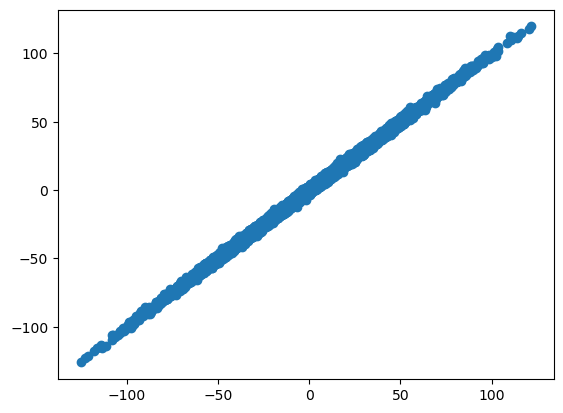
\includegraphics[width=10cm]{homework/homework_8/images/h8_2.png}
    \item so we can see here that plotting a scatter plot of $\Tilde{y}$ broadly looks like a line which makes sense as $\Tilde{y}$ is an affine combination of a signal random variable and noise random variable
\end{itemize}


\item For the $v$ you picked in part $(a)$, sketch some samples of $\rv{y}$ for $d=2$ when $\sigma_{\op{signal}}$ is much smaller than $\sigma_{\op{noise}}$.  
\begin{itemize}
    \color{blue}
    \item \inputminted[firstline=85, lastline=98, breaklines=True]{python}{hw8.py}
    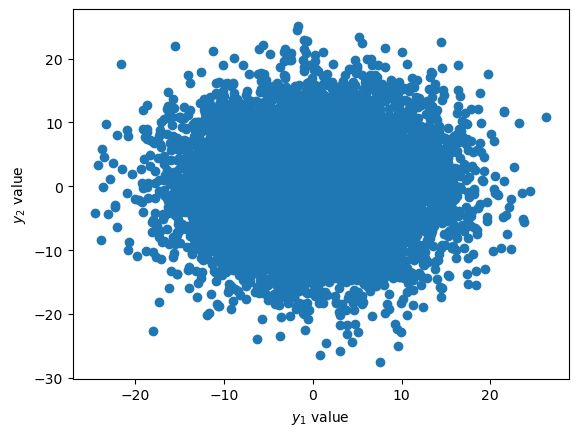
\includegraphics[width=10cm]{homework/homework_8/images/h8_3.png}
    \item here the noise is overpowering the signal so our samples from $\Tilde{y}$ are broadly nomally distributed 
\end{itemize}

\item Is averaging the dataset a good algorithm for estimating $v$?  
\begin{itemize}
  \color{blue}
  \item no averaging the dataset will not get us a good estimate of v
  \item we can examine the expected value of our variables
  \item $E[v\Tilde{x}+\Tilde{z}]=E[v\Tilde{x}]+E[\Tilde{z}]=vE[\Tilde{x}]+E[\Tilde{z}]=v*0+\begin{pmatrix}
    0\\0
  \end{pmatrix}=\begin{pmatrix}
    0\\0
  \end{pmatrix}$
  \item which may not be v
\end{itemize}
\item Compute the covariance matrix of $\rv{y}$. 
\begin{itemize}
  \color{blue}
  \item we can write the variance as $var(\Tilde{y})=E[(\Tilde{y}-E[\Tilde{y}])^2]=E[(\Tilde{x}v+\Tilde{z}-E[\Tilde{x}v+\Tilde{z}])^2]=\\E[(\Tilde{x}v+\Tilde{z}-E[\Tilde{x}]v+E[\Tilde{z}])^2]=
  E[(\Tilde{x}v+\Tilde{z})^2]=E[(\Tilde{x}v)^{t}(\Tilde{x}v)+(\Tilde{x}v)^{t}\Tilde{z}+\Tilde{z}^{t}(\Tilde{x}v)+\Tilde{z}^t\Tilde{z}]=\\
  v^{t}E[\Tilde{x}^{t}\Tilde{x}]v+v^{t}E[\Tilde{x}^{t}\Tilde{z}]+E[\Tilde{z}^{t}\Tilde{x}]v+E[\Tilde{z}^{t}\Tilde{z}]=v^t\sigma_{signal}^{2}v+2v^{t}cov(\Tilde{x},\Tilde{z})+\sigma^{2}_{noise}I\\=v^t\sigma_{signal}^{2}v+\sigma^{2}_{noise}I  $
\end{itemize}
\item Express the eigendecomposition of the covariance matrix in terms of
  $\sigma_{\op{signal}}$, $\sigma_{\op{noise}}$, $v$,
  $u_2$, \ldots, $u_d$.
  Here $u_2$, \ldots, $u_d$ are unit $\ell_2$-norm vectors
  that are orthogonal to $v$ and each other.  
\begin{itemize}
  \color{blue}
  \item given the covariance matrix $v^t\sigma_{signal}^{2}v+\sigma^{2}_{noise}I=\Sigma_{\Tilde{x}}$ 
 \item to find the part that is diagonalizable given our eigenvecotrs wich we can write in matrix form as $P=\begin{pmatrix}
  u_1\\...\\u_n
 \end{pmatrix}$ we first need to think about the eigenvectors of $cov(y)=v^tv\sigma_{singal}^{2}+\sigma^{2}_{noise}I$
 \item we know that the eigenmatrix of $\Lambda =cov(y)$ should eb able to be written as $P\Lambda P^t=cov(y)\Rightarrow \Lambda = P^t cov(y) P$
 \item so doing this out we have $P^{t}(v^t\sigma_{signal}^{2}v+\sigma^{2}_{noise}I)P=\sigma^{2}_{noise}P^tv^tvP+\sigma^{2}_{noise}P^tIP=\sigma^2_{noise}I+\sigma^2_{signal}$
 \item so we can thus write $cov(y)=P(\sigma_{signal}^{2}+\sigma_{noise}^{2}I)$ 
\end{itemize}
\item Suggest an algorithm to estimate the direction of $v$ from the data.  
\begin{itemize}
  \color{blue}
  \item we showed above that $\Sigma_{\Tilde{x}}=v^t\sigma_{signal}^{2}v+\sigma^{2}_{noise}I=cov(y)=P(\sigma_{signal}^{2}+\sigma_{noise}^{2}I)$
  \item so this tells us that we can think of the eigenvalues of our covariance matrix as representing the noise in our data
  \item so thus eigen value i can be expressed as $\lambda_{i}=\sigma^{2}_{signal}+\sigma^{2}_{noise}[i]\Rightarrow \sigma^{2}_{signal}=\lambda[i]-\sigma^{2}_{noise}[i]$
  \item so taking the largest eigenvalue of $cov(y)$ will give us our best estimate of v
\end{itemize}

\end{enumerate}
\newpage
\item (Financial data) In this exercise you will use the code in the findata folder.
  For the data loading code to work properly, make sure you
  have the pandas Python package installed on your system.

  Throughout, we will be using the data obtained by calling
 \verb|load_data()| in \verb|findata_tools.py|.  This will
  give you the names, and closing prices for a set of 18 stocks over a
  period of 433 days ordered chronologically.
  For a fixed stock (such as msft), let
  $P_1,\ldots,P_{433}$ denote its sequence of closing prices ordered in
  time.  For that stock, define the daily returns series $R_i:=P_{i+1}-P_i$ for
  $i=1,\ldots,432$.  Throughout we think of the daily stock returns as features,
  and each day (but the last) as a separate datapoint in $\R^{18}$.
  That is, we have $432$ datapoints each having $18$ features.
  \begin{enumerate}
  \item Looking at the first two principal directions of the
    centered data, give the two stocks with the largest
    coefficients (in absolute value) in each direction.  
    Give a hypothesis why these two stocks have the largest
    coefficients, and confirm your hypothesis using the data.  The file 
 \verb|findata_tools.py| has \verb|pretty_print()|
    functions that can help you output your results.
    You are not required to include the principal directions in
    your submission.
\begin{itemize}
  \color{blue}
  \item call out dataset X
  \item so first of all we need to center our data set $ct(X)=X-m(x)$
  \item then we can find the principal two directions of our data set as the eigenvectors associated to the two largest eigenvalues of our centered dataset 
  \item our first principal direction is  \begin{center}
    \begin{tabular}{c|c|c|c|c|c}
    AAPL & AMZN & MSFT & GOOG & XOM & APC\\
    -0.0017 & -0.1677 & -0.0881 & 0.0273 & -0.1187 & -0.6221\\
    \hline
    CVX & C & GS & JPM & AET & JNJ\\
    -0.1469 & 0.3501 & 0.0950 & -0.0074 & 0.1215 & 0.5089\\
    \hline
    DGX & SPY & XLF & SSO & SDS & USO\\
    -0.0340 & 0.0194 & 0.0822 & 0.0343 & -0.0513 & -0.3511\\
    \end{tabular}
    \end{center}
  \item our second principal direction is \begin{center}
    \begin{tabular}{c|c|c|c|c|c}
    AAPL & AMZN & MSFT & GOOG & XOM & APC\\
    -0.2615 & -0.2632 & -0.2753 & -0.2730 & -0.1138 & -0.1009\\
    \hline
    CVX & C & GS & JPM & AET & JNJ\\
    -0.2414 & -0.2276 & -0.1361 & -0.2734 & -0.2721 & -0.1669\\
    \hline
    DGX & SPY & XLF & SSO & SDS & USO\\
    -0.1354 & -0.2819 & -0.2701 & -0.2814 & 0.2802 & -0.2350\\
    \end{tabular}
    \end{center}
  \item this shows that in both case amazon and google have the largest variance
  \item 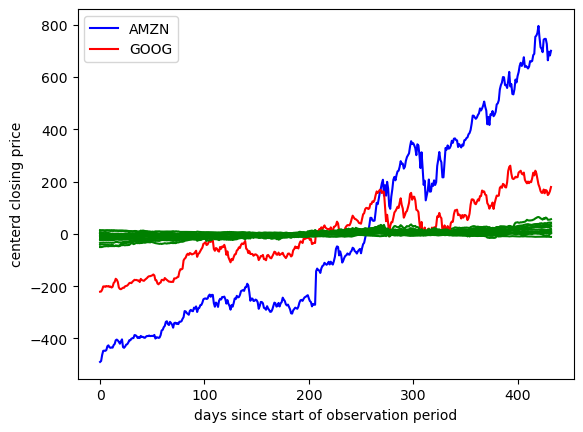
\includegraphics[width=10cm]{homework/homework_8/images/h8_1.png}
    \item in the above graph i plotted the stock price changes of all stocks in the centered dataset over the time period
    \item Amzn is plotted in blue and GOOG is plotted in red, all other stocks are plotted in green 
    \item this confirms out hypothesis as these two stocks very clearly account for the majority of the variance in the dataset. 
    \item here is the code used for this problem.
    \item \inputminted[firstline=118, lastline=175, breaklines=True]{python}{hw8.py}
\end{itemize}
    
  \item Standardize the centered data so that each stock (feature) has
    variance 1 and compute the first 2 principal directions.  This is
    equivalent to computing the principal directions of the
    correlation matrix (the previous part used the covariance
    matrix).  Using the information in the comments of
   \emph{generate\_findata.py} as a guide to the stocks, 
    give an English interpretation of the first 2 principal directions
    computed here. 
    You are not required to include the principal directions in
    your submission.
    \begin{itemize}
     \color{blue}
      \item we can Standardize our data X as
      \item so our first principal direction is \begin{center}
        \begin{tabular}{c|c|c|c|c|c}
        AAPL & AMZN & MSFT & GOOG & XOM & APC\\
        -0.0017 & -0.1677 & -0.0881 & 0.0273 & -0.1187 & -0.6221\\
        \hline
        CVX & C & GS & JPM & AET & JNJ\\
        -0.1469 & 0.3501 & 0.0950 & -0.0074 & 0.1215 & 0.5089\\
        \hline
        DGX & SPY & XLF & SSO & SDS & USO\\
        -0.0340 & 0.0194 & 0.0822 & 0.0343 & -0.0513 & -0.3511\\
        \end{tabular}
        \end{center}
        \item this seems to Suggest that on the Standardized dataset C that is citigroup and JNJ (johnson and johnson) have the most variance 
      \item our second principal direction is \begin{center}
        \begin{tabular}{c|c|c|c|c|c}
        AAPL & AMZN & MSFT & GOOG & XOM & APC\\
        -0.2615 & -0.2632 & -0.2753 & -0.2730 & -0.1138 & -0.1009\\
        \hline
        CVX & C & GS & JPM & AET & JNJ\\
        -0.2414 & -0.2276 & -0.1361 & -0.2734 & -0.2721 & -0.1669\\
        \hline
        DGX & SPY & XLF & SSO & SDS & USO\\
        -0.1354 & -0.2819 & -0.2701 & -0.2814 & 0.2802 & -0.2350\\
        \end{tabular}
        \end{center}
        \item this seems to Suggest State Street's SPDR S&P 500 ETF has the largest coefficient of negative variance on our Standardized data set 
        \item and SDS ProShares inverse levered ETF has the largest positive coefficient of variance
    \item a lot of the code from the last question stays the same, but i will include the standardize function 
    \item \inputminted[firstline=178, lastline=182, breaklines=True]{python}{hw8.py}
    \end{itemize}
  \item Assume the stock returns each day are drawn independently from a
    multivariate distribution $\rx$ where
    $\rx[i]$ corresponds to the $i$th stock.  Assume further that
    you hold a portfolio with $200$ shares of each of appl, amzn, msft, and
    goog, and $100$ shares of each of the remaining 14 stocks in the
    dataset.  Using the sample covariance matrix as an estimator for
    the true covariance of $\rx$, approximate the standard deviation of
    your 1 day portfolio returns $\ry$ (this is a measure of the risk of your
    portfolio).  Here $\ry$ is given by
    $$\ry := \sum_{i=1}^{18} \alpha[i] \rx[i],$$
    where $\alpha[i]$ is the number of shares you hold of stock $i$.
    
  \begin{itemize}
    \color{blue}
    \item assume the random vector for stock return (in terms of dollars is) $\Tilde{x}=\begin{pmatrix}
      'aapl',\\
      'amzn',\\
      'msft',\\
      'goog',\\
      'xom', \\
      'apc',  \\
      'cvx', \\
      'c',    \\
      'gs',  \\
      'jpm', \\
      'aet', \\
      'jnj',  \\
      'dgx',\\
      'spy',  \\
      'xlf',\\
      'sso',  \\
      'sds',  \\
      'uso', \\
    \end{pmatrix}$ 
    \item so our alpha vector is given by $\alpha=\begin{pmatrix}
      200,\\
      200,\\
      200,\\
      200,\\
      100\\100\\100\\100\\100\\100\\100\\100\\100\\100\\100\\100\\100\\100
    \end{pmatrix}$
    \item we are told that $\Tilde{y}=\Sigma_{i=1}^{n}\alpha[i]\Tilde{x}[i]$
    \item this is a linear combination of $\Tilde{x}$ so we know that $var(\Tilde{y})=var(\Sigma_{i=1}^{18}\alpha^{t}\Tilde{x}_i)=\Sigma_{i=1}^{18}\alpha^{t}\Sigma_{X}[i]\alpha=\alpha^{t}\Sigma_{X}\alpha=12554439583.358356$  which is a lot of variance 
  \end{itemize}
  \item Assume further that $\rx$ from the previous part has a
    multivariate Gaussian distribution.  Compute the probability
    of losing $1000$ or more dollars in a single day.  That is,
    compute
    $$\Pr(\ry \leq -1000).$$
  \end{enumerate}
\begin{itemize}
 \color{blue}
  \item we are told that $\Tilde{x}$ is normally distributed, that is $\Tilde{x}\sim \mathcal{N}(\mu, \Sigma_{\Tilde{x}})$ 
  \item so we want to reason about $\Tilde{y}=\alpha^{t}\Tilde{x}$
  \item we know that $E[\tilde{y}]=E[\alpha^{t}\Tilde{x}]=\alpha^{t} E[\Tilde{x}]=\alpha^{t} \mu$
  \item and can see that $var(\Tilde{y})=E[(\Tilde{y}-E[\Tilde{y}])^2]=E[(\alpha^{t} \Tilde{x}-\alpha^{t}\mu)^2]=E[(\alpha^{t}( \Tilde{x}-\mu))((\alpha^{t}( \Tilde{x}-\mu)))^t]=E[\alpha^{t}(\Tilde{x}-\mu)((\Tilde{x}-\mu)^{t}\alpha)]=\alpha^{t}E[(\Tilde{x}-\mu)((\Tilde{x}-\mu)^{t})]\alpha=\alpha^{t}\Sigma_{x}\alpha$
 
  \item we can define $ct(\Tilde{y}):=\Tilde{y}-E[\tilde{y}]$
  \item we can see that $E[ct(\Tilde{y})]=E[\Tilde{y}-E[\Tilde{y}]]=E[\Tilde{y}]-E[\Tilde{y}]=0$
  \item and $var(ct(\Tilde{y}))=E[ct(\Tilde{y})-E[(ct(\Tilde{y})])^2]=E[ct(\Tilde{y})^2]=E[(\Tilde{y}-E[\Tilde{y}])^2]=\alpha^{t}\Sigma_{\Tilde{x}}\alpha$
  \item so in other words we know $ct(\Tilde{y})\sim\mathcal{N}(0,\alpha^{t}\Sigma_{\Tilde{x}}\alpha)$
  \item so thus we are dealing with gaussian random variable as opposed to a gaussian random vector
  \item we can see thus that $P(\Tilde{y}\leq -1000)=1-F_{\Tilde{y}}(-1000)=.5$
  \item so we have a 50\%  chance of losing more than 1000 dollars with this strategy 
  \item here is the code for this question 
  \item \inputminted[firstline=223, lastline=227, breaklines=True]{python}{hw8.py}
\end{itemize}


  Note: The assumptions made in the previous parts are often
  invalid and can lead to inaccurate risk calculations in real
  financial situations. 

\end{enumerate}
\end{document}
